\documentclass[journal, 11pt]{IEEEtran}

% *** CITATION PACKAGES ***
%
%\usepackage{cite}https://www.overleaf.com/project/5d8e32cf8b64620001d24060
\usepackage{capt-of}%%To get the caption
\usepackage{gensymb}
\usepackage{graphicx} %package to manage images
\graphicspath{ {./images/} }
\usepackage{wrapfig}

\usepackage{amsmath}
\usepackage{amssymb}

\usepackage{lipsum}

\usepackage[style=ieee]{biblatex}
\DeclareLanguageMapping{english}{english-apa}
\addbibresource{references.bib}
\usepackage[justification=centering]{caption}

\usepackage{setspace}

\usepackage{hhline}


\usepackage{changepage} 

\usepackage{booktabs}
\usepackage{xcolor}

\usepackage{makecell}
\usepackage{graphicx,subcaption}
\usepackage{listings}
\renewcommand\theadfont{}
\DeclareMathOperator{\EX}{\mathbb{E}}% expected value


\usepackage{multicol} 

\raggedbottom

\begin{document}


\pagenumbering{gobble}
%\clearpage\mbox{} % adds and empty page
%\clearpage
\pagenumbering{arabic}
\setcounter{page}{1}

\title{\LARGE{Flyway: Predicting Foot Traffic in Open Spaces on Campus}}

\author{ ENGR-UH 4560 Machine Learning, Fall 2019\\
\medskip
Nishant Aswani,~\IEEEmembership{nsa325@nyu.edu}
Barkin Simsek,~\IEEEmembership{bs3528@nyu.edu}}% <-this % stops a space


% The paper headers
\markboth{Aswani, Simsek ENGR-UH 4560 Machine Learning, Fall 2019}%
{}

% make the title area
\maketitle

% As a general rule, do not put math, special symbols or citations
% in the abstract or keywords.
% \begin{abstract}


% \end{abstract}

%%%%%%%%%%%%%%%%%%
%% Introduction %%
%%%%%%%%%%%%%%%%%%
\section{Introduction}
\subsection{Motivation}
\IEEEPARstart{P}\lowercase{redicting} traffic is one of the most common timeseries forecasting problems available for tackling. When placed in the context of smart cities, the problem is motivated by the question of "how to enable users to make smarter choices when using transportation networks" \cite{lv2014traffic}. However, this can be broadened to include how smart choices are made for using infrastructure and public spaces in general. \\

\noindent Given that our campus has multiple open spaces for students to study and/or relax, we want to be able to forecast the foot traffic that occurs in the multiple spaces. This could eventually be furthered, and the information organized, to provide a live prediction visualization of foot traffic around campus.

\subsection{Problem Statement}

\noindent Gathering from our previous experience with the New York City (NYC) taxi data set, we had a rough idea on how to approach timeseries data, along with the models and analysis that is carried out on such data. We were able to draw parallels between foot traffic in our project to pickup counts in certain locations in NYC.

%%%%%%%%
% NOTE %
%%%%%%%%
% include info about how we gather the data, why we gather the data that way, and why we get that specific data or those features

\section{Existing Literature and Body of Work}

\subsection{Waitz: Know Before You Go}

\noindent One of the inspirations of this project was the Waitz application developed by students at University of California San Diego (UCSD) \cite{waitz}. They used Raspberry Pi's, loaded with network monitoring firmware and placed at various locations around their campus, to approximate the number of students within a given area. They did so by logging the Bluetooth and MAC addresses of devices within range of the network sniffing Pis.\\

% \begingroup
%     \centering
%     \medskip
%     %width=\columnwidth
%     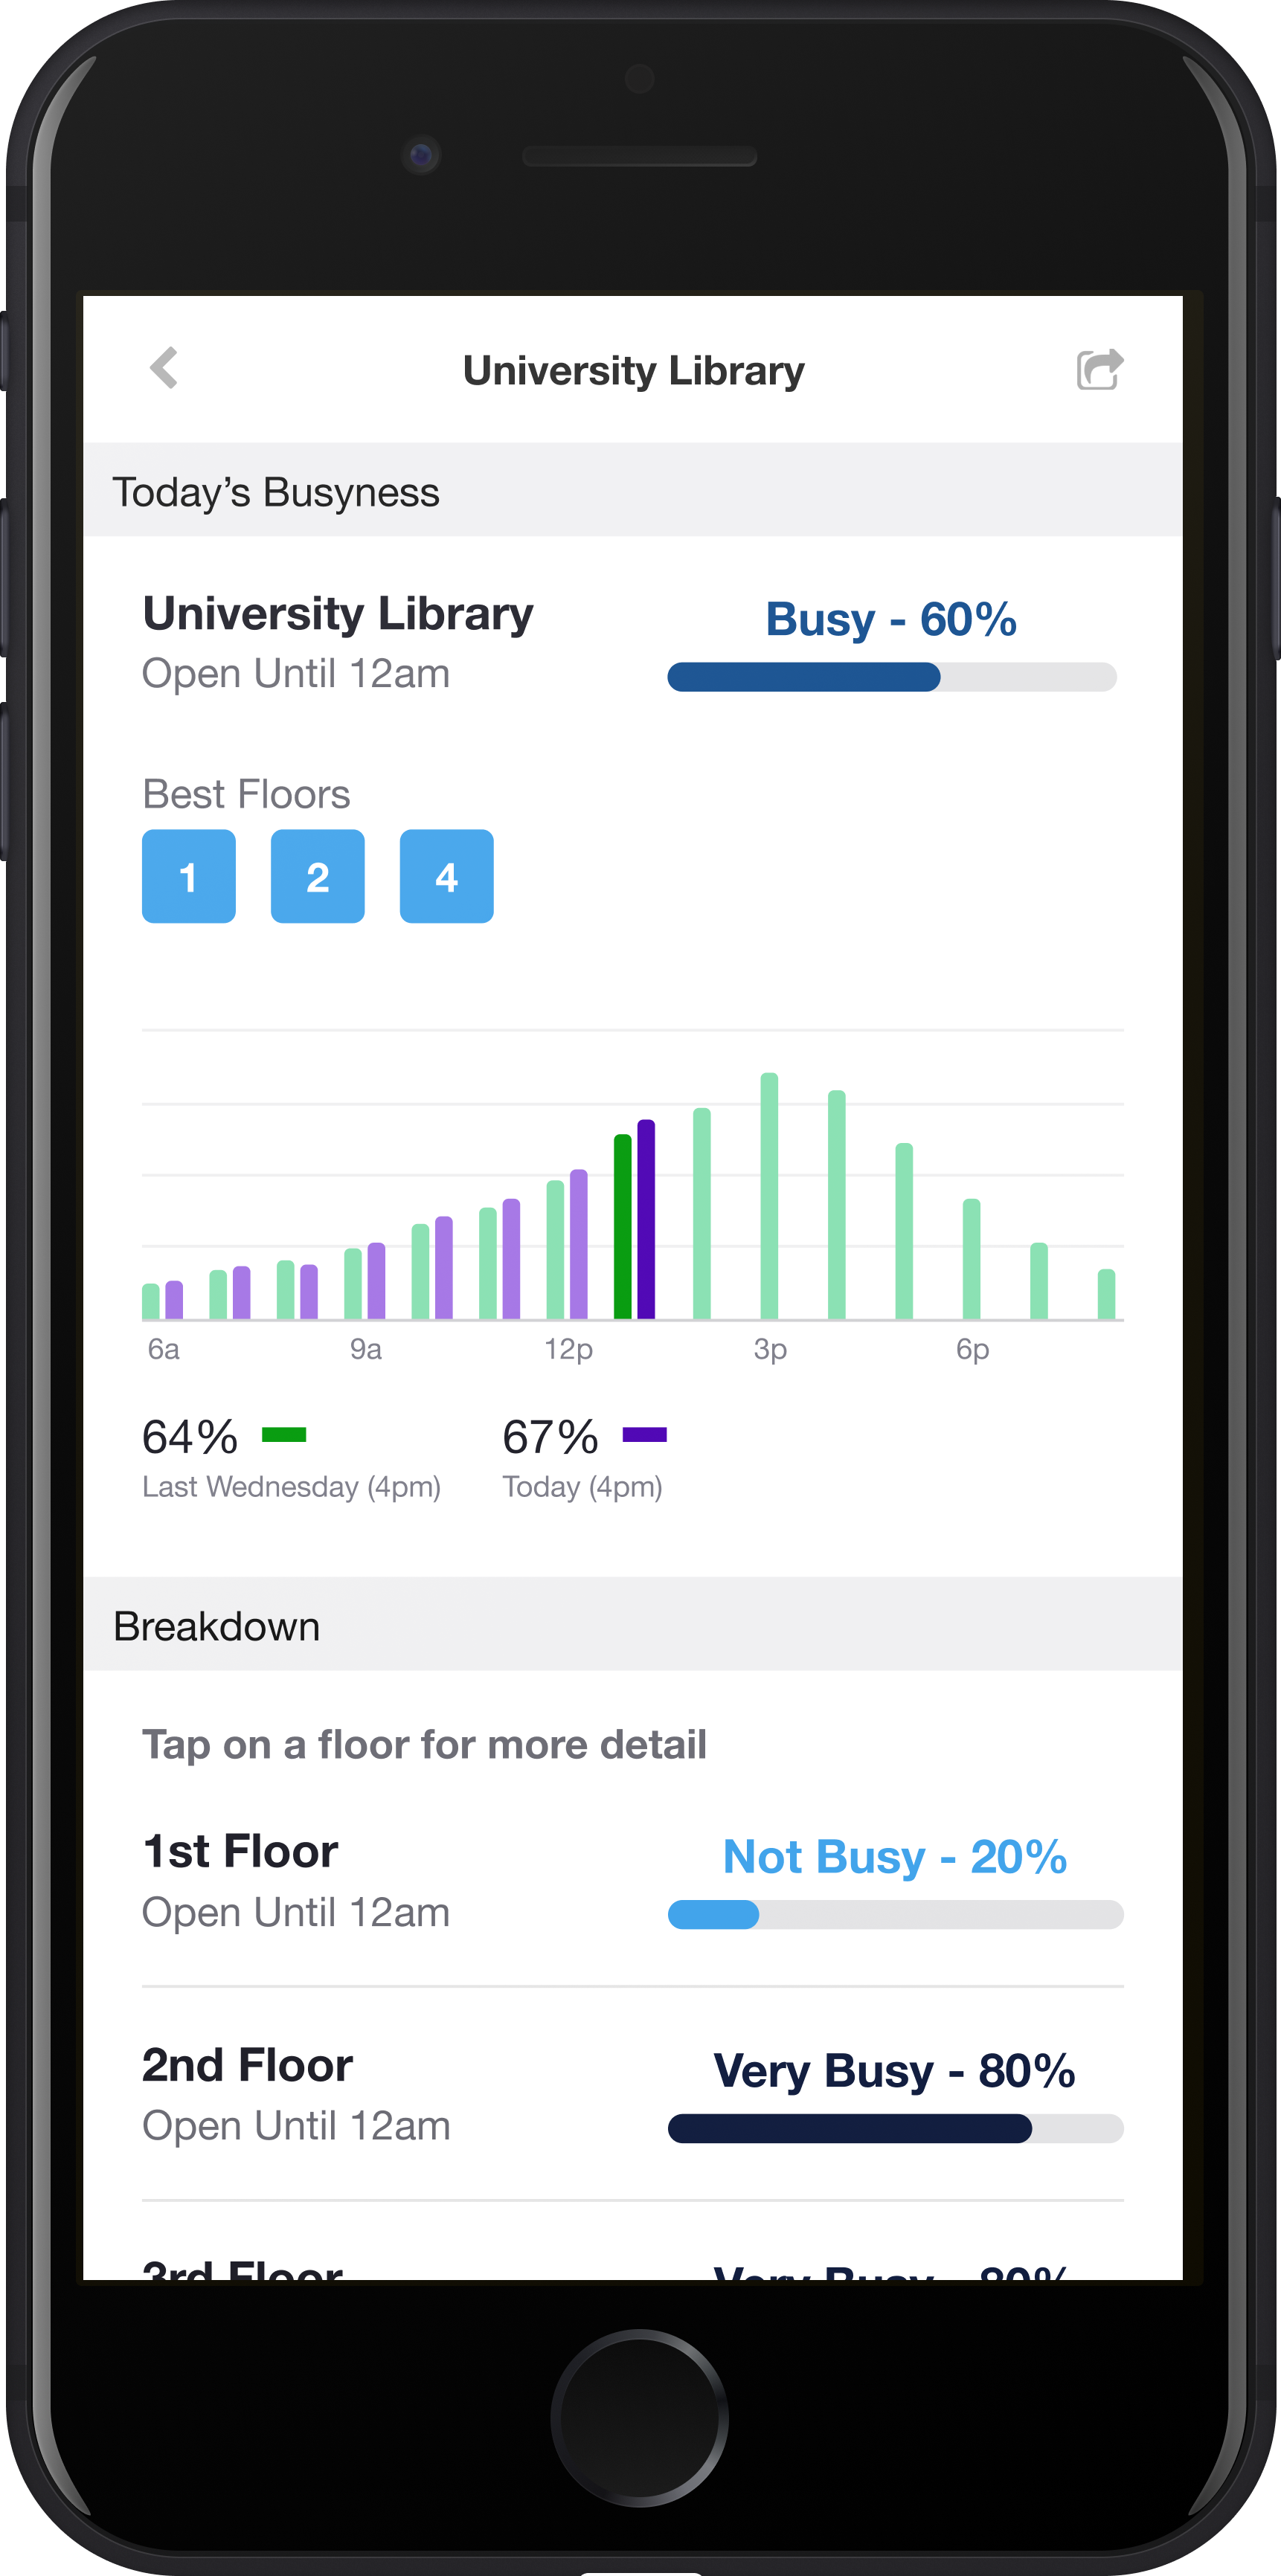
\includegraphics[width=0.4\columnwidth]{./images/waitz.png}
%     \captionof{figure}{Waitz UI}
%     \label{fig:waitz_ui}
%     \medskip
% \endgroup
% \medskip

\noindent However, their application is relatively simple as they did not use this data to forecast the "busyness" of locations or make predictions. Instead, it seems that they focused more on data collection and visualization. As a result, we thought it would be interesting to implement a similar tool for our campus; in the process, we hoped discover if there are any timeseries patterns we can exploit to provide useful information for students. \\


\section{Methodology}


\begin{itemize}
    \item frame.number
    \item frame.time
    \item wlan.addr
    \item wlan.ta
    \item wlan.ra
    \item wlan.sa
    \item wlan.da
    \item wlan.bssid
    \item wlan.fc.type
    \item wlan.fc.type\_subtype
    \item radiotap.channel.freq
    \item radiotap.datarate
    \item radiotap.dbm\_antsignal
\end{itemize}


\subsection{Feasibility}


%%%%%%%%
% NOTE %
%%%%%%%%
% include information about some nuances we need to think about or we can extract. For example, do we have to worry about someone "passing by" if their MAC address was available for just a small bit of time. 




\subsection{Applicability to Solving the Problem}


%%%%%%%%%%%%%%%%%%%%%%%%%
%% Experimental Method %%
%%%%%%%%%%%%%%%%%%%%%%%%%

%%%%%%%%%%%%%
%% Results %%
%%%%%%%%%%%%%

%%%%%%%%%%%%%%%%
%% Discussion %%
%%%%%%%%%%%%%%%%



\end{document}

%%%%%%%%%%%%%%%
%% Equations %%
%%%%%%%%%%%%%%%

% \begin{equation}
%     \begin{split}
%         X &\texttt{\char`\~} Poisson(\lambda) \\
%         \\
%         P(X=k) &= \frac{\lambda^k e^{-\lambda}}{k!} \\
%         \\
%         \EX(k) &= e^{-\lambda}\sum_{k=1}^{\infty} \frac{\lambda^n}{(n-1)!}\\
%         \\
%         &= e^{-\lambda}\lambda\sum_{k=1}^{\infty} \frac{\lambda^{k-1}}{(k-1)!}\\
%         \\
%         &= e^{-\lambda}\lambda\sum_{n=0}^{\infty} \frac{\lambda^{n}}{(n)!}\\
%         \\
%         &= e^{-\lambda}\lambda e^{\lambda} = \lambda\\
%     \end{split}
%     \label{eq:mutual}
% \end{equation}

% \noindent Hence, we know that the $\lambda$ parameter can be approximated as the mean degree.

% \begin{equation}
%     \begin{split}
%         \lambda = \frac{\sum_{i=1}^{n}D_i}{n}
%     \end{split}
%     \label{eq:poisson_distribution}
% \end{equation}

%%%%%%%%%%%
%% Table %%
%%%%%%%%%%%

% \begingroup
%     \medskip
%     \centering
%     \def\arraystretch{1.5}
%         \begin{tabular}{lcc}
%             \toprule
%             & Random Network & Scale-Free Network \\
%             \midrule
%             Avg. of Avg. Degree    & 3.9988    &  4.0035   \\
%             Var. of Avg. Degree    & 7.6800$\times 10^{-7}$ & 3.1156$\times 10^{-6}$  \\
%             Avg. of Avg. Distance  & 5.5694 & 5.0935    \\
%             Var. of Avg. Distance  & 1.5507 & 0.5377   \\
%             \bottomrule
%         \end{tabular}
%     \captionof{table}{Statistics of fifty runs where \\ n = 5,000, e = 10,000}
%     \label{table:fifty_runs}
%     \medskip
% \endgroup
